\documentclass[a4paper,11pt]{article}
\pdfoutput=1 % if your are submitting a pdflatex (i.e. if you have
             % images in pdf, png or jpg format)

\usepackage{jcappub} % for details on the use of the package, please
                     % see the JCAP-author-manual

\usepackage[T1]{fontenc} % if needed
\usepackage[utf8]{inputenc}

%Good vectors
\usepackage{esvect}
\renewcommand*\vec{\vv}

%QFT
\usepackage{slashed}


\usepackage{subcaption}


\renewcommand{\O}{\Omega}
\newcommand{\ex}{\text{e}}

%Equations
\newcommand\numberthis{\addtocounter{equation}{1}\tag{\theequation}}

%correct i.e.
\usepackage{xspace}
\newcommand*{\ie}{i.e., }
\newcommand*{\eg}{e.g., }
\newcommand*{\fig}{Fig.\@\xspace}
\newcommand*{\Eq}{Eq.\@\xspace}
\newcommand*{\Eqs}{Eqs.\@\xspace}

%Integrals
\usepackage{xifthen}% Provides \isempty test
\newcommand*\diff{\mathrm{d}} % Straight differential
\newcommand*\ldiff[2][]{ \ifthenelse{\isempty{#1}}{ \diff #2}{\diff^#1#2} \,} % Differential with measure; the mandatory argument is the name of the measure, the option one is the dimension
\let\limitint\int % Only when I provide explicit limits for the integration, I need to do the spacing myself
\renewcommand{\int}{\limitint \!} % The standard integral should have correct spacing




\title{  title  title  title  title  title  title  title  title }
\author[a]{  author  author  author }
\author[a]{  author  author  author }
\author[a]{  author  author }
\affiliation[a]{  author  author  author  author  author  author  author  author  author  author  author  \'Ecole  author  author  author \'ed\'erale  author  author  author  author  author  author  author }
\emailAdd{  author  author  author  author }
\emailAdd{  author  author  author  author }
\emailAdd{  author  author  author  author }

\abstract{
  abstract  abstract  abstract  abstract  abstract  abstract  abstract  abstract  abstract  abstract  abstract  abstract  abstract  abstract  abstract  abstract  abstract  abstract  abstract  abstract  abstract  abstract  abstract  abstract  abstract  abstract  abstract  abstract  abstract  abstract  abstract  abstract  abstract  abstract  abstract  abstract  abstract  abstract  abstract  abstract  abstract  abstract  abstract  abstract  abstract  abstract  abstract  abstract  abstract  abstract  abstract  abstract  abstract  abstract  abstract  abstract  abstract  abstract  abstract  abstract  abstract  abstract  abstract  abstract  abstract   abstract  abstract  abstract  abstract  abstract  abstract  abstract  abstract  abstract  abstract   abstract  abstract  abstract  abstract  abstract  abstract  abstract  abstract  abstract   abstract  abstract   abstract  abstract  abstract  abstract   abstract  abstract  abstract  abstract  abstract  abstract  abstract  abstract  abstract  abstract  abstract  abstract  abstract  abstract  abstract  abstract  }



\begin{document}
\maketitle
\flushbottom

\section{  section  section }
\label{sec:introduction}
  column 1  column 1  column 1  column 1  column 1  column 1  column 1  column 1  column 1  column 1  column 1  column 1  column 1  \cite{1207.7214, 1207.7235}  column 1  column 1  column 1  column 1  column 1 \cite{Englert:1964et, Higgs:1964ia, Higgs:1964pj}  column 1  column 1  column 1  column 1  column 1  column 1  column 1  column 1  column 1  column 1 \cite{1001.4538, 1807.06211}  column 1  column 1  column 1  column 1  column 1  column 1  column 1  column 1 \cite{Starobinsky:1980te, Guth:1980zm, Linde:1981mu, Mukhanov:1981xt}  column 1  column 1  column 1  column 1  column 1  column 1  column 1  column 1  column 1  column 1  column 1  column 1  column 1  column 1  column 1  column 1 \cite{0710.3755}  column 1  column 1  column 1  column 1  column 1  column 1  column 1  column 1  column 1  column 1  column 1  column 1  column 1  column 1     column 1  column 1  column 1  column 1  column 1  column 1  column 1  column 1  column 1  column 1 \cite{0710.3755}  column 1  column 1  column 1  column 1  column 1 \cite{0803.2664}  column 1 \footnote
%
{See \cite{1807.02376} and \cite{2001.10135} for reviews of metric and Palatini Higgs inflation, respectively.}
% 
  column 1  column 1  column 1  column 1  column 1  column 1  
  column 1   column 1  column 1  column 1  column 1   column 1  column 1  column 1   column 1  column 1  column 1  column 1  column 1  column 1   column 1  column 1  column 1  column 1  column 1  column 1  column 1  column 1  column 1  column 1 \footnote
	%
	{Note that even if there were no such coupling at tree level, it would be generated by quantum corrections \cite{Callan:1970ze}.
	}
	%
  column 1  column 1  column 1  column 1  column 1  column 1  column 1  column 1  column 1  column 1  column 1  column 1  column 1 \cite{0710.3755}  column 1  column 1  column 1  column 1  column 1  column 1 \ie  column 1  column 1  column 1   column 1  column 1  column 1  column 1  column 1 \cite{Palatini19,Einstein25}  column 1  column 1  column 1  column 1   column 1  column 1  column 1  column 1  column 1   column 1  column 1  column 1  column 1  column 1  column 1  column 1  column 1  column 1  column 1  column 1  column 1  column 1  column 1 \eqref{action_full}  column 1  column 1  column 1  column 1  column 1  column 1  column 1  column 1  column 1  column 1  column 1  column 1 \cite{0803.2664}  column 1  column 1  column 1 \textit{Palatini Higgs inflation}  column 1  column 1  column 1  column 1  column 1 \textit{metric Higgs inflation.}
  column 1  column 1    column 1  column 1  column 1  column 1  column 1  column 1  column 1  column 1  column 1  column 1   column 1  column 1  column 1  column 1  column 1  column 1  column 1  column 1  column 1  column 1  column 1  column 1  column 1  column 1  column 1  column 1  column 1  column 1   column 1  column 1  column 1  column 1   column 1  column 1  column 1  column 1  column 1  column 1   column 1  column 1  column 1  column 1  column 1  column 1  column 1  column 1  column 1  column 1  column 1  column 1  column 1  column 1  column 1  column 1  column 1    column 1  column 1  column 1  column 1  column 1  column 1  column 1  column 1  \cite{0803.2664}  column 1  column 1  column 1  column 1  column 1  column 1  column 1  column 1  column 1  column 1  column 1  column 1  \cite{1807.06211}  column 1 \footnote
%
{See \cite{1303.3787} for a review of various inflationary models and their compatibility with measurements.}
%
  column 1  column 1  column 1  column 1  column 1  column 1  column 1  column 1  column 1  column 1  column 1  column 1  column 1  column 1  column 1    column 1  column 1  column 1  column 1  column 1  column 1  column 1  column 1  column 1  column 1  column 1  column 1  column 1  column 1  column 1  column 1  column 1  column 1  column 1  column 1  column 1  column 1  column 1  column 1  column 1  column 1  column 1  column 1  column 1  column 1  column 1  column 1  column 1  column 1  column 1  column 1  column 1  column 1  column 1  column 1  column 1  column 1 \cite{1008.5157}  column 1     column 1  column 1  column 1  column 1  column 1  column 1  column 1  column 1  column 1   column 1  column 1  column 1  column 1  column 1  column 1  column 1  column 1  column 1  column 1  column 1  column 1  column 1  column 1  column 1   column 1  column 1  column 1  column 1  column 1  column 1  column 1   column 1  column 1  column 1  column 1  column 1  column 1  column 1  column 1  column 1  column 1  column 1  column 1  column 1  column 1  column 1   column 1  column 1  column 1  column 1  column 1  column 1  column 1  column 1  column 1  column 1  column 1  column 1   column 1   column 1    column 1  column 1  column 1  \cite{0902.4465,0903.0355}  column 1  column 1  column 1 \cite{1012.2900}  column 1  column 1 \footnote
%
{Also in the metric theory of gravity, there are proposals to increase $\Lambda$ without introducing new degrees of freedom \cite{1003.2635, 1005.2978}. They rely on higher-dimensional operators. The perturbative cutoff in the theory studied in \cite{1003.2635} was further discussed in \cite{1612.06253, 1711.08761}.}
%
  column 1  column 1  column 1  column 1  column 1  column 1  column 1  column 1  column 1   column 1  column 1  column 1   column 1  column 1  column 1  column 1  column 1  column 1  column 1  column 1  column 1  column 1  column 1  column 1  column 1  column 1     column 1  column 1  column 1  column 1  column 1  column 1  column 1  column 1  column 1  column 1  column 1  column 1  column 1  column 1  column 1  column 1  column 1  column 1  column 1  column 1  column 1   column 1  column 1 \cite{1008.5157}  column 1     column 1  column 1  column 1  column 1  column 1  column 1  column 1  column 1  column 1  column 1  column 1  column 1  column 1  column 1  column 1  column 1  column 1 \cite{1609.05209, 1610.08916}  column 1  column 1  column 1  column 1  column 1   column 1  \cite{1008.5157, 1412.3811}  column 1  column 1  column 1  column 1  column 1  column 1  column 1  column 1  column 1  column 1  column 1  column 1  column 1  column 1  column 1  column 1  column 1  column 1  column 1  column 1  column 1  column 1  column 1  column 1  column 1  column 1  column 1  column 1  column 1 \cite{1609.05209, 1610.08916}  column 1 \footnote
%
{For earlier studies of preheating in metric Higgs inflation see \cite{0812.3622, 0812.4624}.}
%
  column 1  column 1  column 1  column 1  column 1  column 1  column 1  column 1  column 1  column 1  column 1  column 1  column 1  column 1  column 1  column 1  column 1  column 1  column 1  column 1  column 1  column 1  column 1 \cite{1902.10148}  column 1   
  column 1  column 1  column 1  column 1  column 1  column 1   column 1  column 1  column 1  column 1  column 1  column 1  column 1  column 1  column 1  column 1  column 1  column 1  column 1  column 1  column 1  column 1  column 1  column 1  column 1  column 1  column 1  column 1  column 1 \cite{1010.1417, 1307.5298, 1501.02231, 1701.07665}  column 1  column 1  column 1  column 1  column 1  column 1  column 1  \cite{1008.5157,Aydemir:2012nz}  column 1  column 1  column 1  column 1  column 1  column 1  column 1  column 1  column 1  column 1  column 1  column 1  column 1  column 1  column 1  column 1  column 1  column 1  column 1  column 1  column 1  column 1  column 1  column 1  column 1  column 1  column 1  column 1  column 1  column 1  column 1  column 1  column 1  column 1  column 1  column 1  column 1  column 1  column 1  column 1  column 1  column 1  column 1  column 1  column 1  column 1  column 1  column 1  column 1  column 1  column 1  column 1  column 1  column 1  column 1  column 1  column 1  column 1  column 1  column 1  column 1  column 1  column 1  column 1  column 1  column 1  column 1  column 1 \cite{1008.5157}  column 1  column 1  column 1  column 1 \cite{1412.3811}  column 1  column 1  column 1  column 1  column 1  column 1  column 1  column 1  column 1  column 1  column 1  column 1  column 1  column 1  column 1   
  column 1  column 1  column 1  column 1  column 1  column 1  column 1   column 1  column 1  column 1  column 1  column 1  column 1  column 1  column 1  column 1  column 1  column 1  column 1  column 1  column 1  column 1  column 1  column 1  column 1  column 1  column 1  column 1  column 1  column 1  column 1  column 1  column 1  column 1   column 1   column 1  column 1  column 1  column 1  column 1  column 1  column 1  column 1  column 1  column 1  column 1  column 1  column 1  column 1  column 1  column 1  column 1  column 1 \cite{1008.5157,1403.6078,1412.3811,Enckell:2016xse, 1706.05007}  column 1  column 1  column 1  column 1  column 1  column 1  column 1  column 1  column 1  column 1  column 1  column 1  column 1  column 1  column 1  column 1  column 1  column 1  column 1  column 1  column 1  column 1  column 1  column 1  column 1  column 1 \cite{0904.1537}  column 1  column 1  column 1  column 1   column 1  column 1  column 1  column 1  column 1  column 1  column 1  column 1  column 1  column 1   column 1  column 1  column 1  column 1  column 1  column 1  column 1  column 1  column 1  column 1  column 1  column 1  column 1  column 1   column 1  column 1  column 1  column 1  column 1  column 1  column 1  column 1  column 1  column 1   column 1  column 1  column 1  column 1  column 1  column 1  column 1  column 1  column 1  column 1  column 1  column 1  column 1  column 1  column 1  column 1  column 1  column 1  column 1  column 1  column 1   column 1  column 1  column 1  column 1  column 1  column 1  column 1  column 1  column 1 \cite{0812.4950, 0904.1537,1411.1923}  column 1 \footnote
%
{See also \cite{0809.2104, 0812.4946, 0904.1698, 0910.1041} for early studies of quantum effects in Higgs inflation.}
%
  column 1  column 1  column 1  column 1  column 1  column 1  column 1  column 1  column 1  column 1  column 1  column 1  column 1  column 1  column 1  column 1  column 1  column 1  column 1  column 1  column 1  column 1  column 1  column 1  column 1  column 1  column 1  column 1  column 1  column 1  column 1  column 1  column 1  column 1  column 1  column 1  column 1  column 1  column 1  \footnote
%
{Other aspects of quantum effects in Palatini Higgs inflation have been considered in \cite{1709.07853,1712.04874, 1802.09299}.}
%
  column 1  column 1  column 1  column 1  column 1  column 1  column 1  column 1  column 1  column 1  column 1   column 1  column 1  column 1  column 1  column 1  column 1  column 1  column 1  column 1  column 1  column 1   column 1  column 1  column 1  column 1  column 1  column 1  column 1  column 1   column 1  column 1  column 1  column 1  column 1  column 1   column 1  column 1  column 1  column 1     column 1  column 1  column 1  column 1  column 1  column 1  column 1   column 1  column 1  column 1  column 1  column 1  column 1  column 1  column 1  column 1  column 1 \cite{1012.2900}  column 1  column 1  column 1  column 1  column 1  column 1   column 1  column 1  column 1  column 1  column 1  column 1  column 1  column 1  column 1  column 1  column 1  column 1  column 1  column 1  column 1  column 1  column 1  column 1  column 1  column 1  column 1  column 1 \ie  column 1  column 1  column 1  column 1  column 1  column 1  column 1  column 1  column 1  column 1  column 1  column 1  column 1  column 1  column 1  column 1  column 1  column 1  column 1   column 1  column 1  column 1  column 1  column 1  column 1  column 1  column 1  column 1  column 1  column 1  column 1  column 1  column 1    column 1  column 1  column 1  column 1  column 1  column 1  column 1  column 1  column 1  column 1  column 1  column 1  column 1  column 1  column 1  column 1  column 1   
  column 1  column 1  column 1  column 1  column 1  column 1 \ref{sec:review}  column 1  column 1  column 1  column 1  column 1  column 1  column 1  column 1  column 1  column 1  column 1  column 1 \ref{sec:newPhysics}  column 1  column 1  column 1  column 1  column 1  column 1  column 1  column 1  column 1  column 1  column 1  column 1  column 1  column 1  column 1  column 1   column 1  column 1  column 1  column 1  column 1  column 1  column 1  column 1  column 1   column 1  column 1  column 1  column 1  column 1  column 1  column 1  column 1  column 1  column 1  column 1  column 1  column 1  column 1  column 1  column 1  column 1   column 1  column 1  column 1  column 1  column 1  column 1  column 1  column 1  column 1  column 1  column 1  column 1  column 1  column 1  column 1  column 1 \ref{sec:connection}  column 1  column 1  column 1  column 1 \ref{sec:conclusion}  column 1   
\section{  section  section  section  section  section }
\label{sec:review}
  column 1  column 1  column 1  column 1  column 1  column 1  \cite{0710.3755}  column 1  column 1  column 1 \cite{0803.2664}  column 1  column 1  column 1  column 1  column 1  column 1 \ref{action_full}  column 1  
  column 1  column 1  column 1  column 1  column 1  column 1  column 1   column 1  column 1  column 1  column 1  column 1  column 1  column 1  column 1   column 1  column 1  column 1  column 1  column 1  column 1  column 1  column 1   column 1  column 1  column 1  column 1  column 1  column 1  column 1  column 1  column 1  column 1  column 1  column 1  column 1  column 1  column 1   column 1  column 1  column 1  column 1  column 1  column 1  column 1  column 1  column 1  column 1   
  column 1  column 1 \ref{action}  column 1  column 1  
  column 1  column 1  column 1  column 1  column 1  column 1  column 1  column 1  column 1  column 1  column 1  column 1  column 1  column 1  column 1   column 1  column 1  column 1  column 1  column 1  column 1  column 1  column 1  column 1  column 1  column 1   column 1  column 1  column 1  column 1  column 1  column 1  column 1  column 1 \ref{FieldTransform1}  column 1  column 1  column 1   column 1  column 1  column 1 \ref{table}  column 1  column 1  column 1  column 1  column 1  column 1  column 1  column 1  column 1  column 1   column 1  
  column 1  column 1  column 1  column 1  column 1  column 1  column 1   column 1  column 1  column 1  column 1  column 1  column 1  column 1  column 1  column 1  column 1  column 1  column 1 \ref{table}  column 1 \footnote
%
	{Also in the metric scenario, \Eq \eqref{FieldTransform2} can be integrated exactly, giving $\chi$ as a function of $h$ \cite{0812.4624}.}
%
  column 1  column 1  column 1  column 1  column 1   column 1   column 1  column 1  
  column 1  
  column 1  column 1   column 1  column 1  column 1  column 1  column 1  column 1 \ref{table}  column 1  column 1  column 1   column 1   column 1  column 1  column 1  column 1  column 1  column 1  column 1  column 1   column 1  column 1  column 1  column 1  column 1  column 1  column 1  column 1  column 1  column 1  column 1   column 1  column 1  column 1  column 1  column 1  column 1  column 1  column 1  column 1   column 1  column 1  column 1  column 1  column 1  column 1   	\begin{table}
	
	\caption{  caption  caption  caption  caption  caption  caption  caption  caption  caption  caption   caption  caption  caption  caption   caption  caption  caption  caption  caption  caption   caption  caption  caption  caption  caption  caption  caption  caption  caption  caption   caption  caption  caption  caption  caption  caption  caption   caption  caption  caption   caption   caption  caption  caption  caption  caption   caption   caption }
	\label{table}
\end{table}
  column 1  column 1  column 1  column 1  column 1  column 1  column 1  \ref{einsteinAction}  column 1  column 1  column 1  column 1  column 1  column 1  column 1  column 1  column 1  column 1  column 1  column 1  column 1  column 1  
  column 1  column 1 \ref{action}  column 1  column 1  column 1  column 1  column 1  column 1  column 1  column 1  column 1  column 1  column 1  column 1   column 1  column 1  column 1  column 1  column 1  column 1  column 1  column 1  column 1  column 1  column 1  column 1  column 1  column 1  column 1  column 1  column 1  column 1  column 1  column 1  column 1  column 1  column 1  column 1  column 1  column 1  column 1  column 1  column 1  column 1  column 1     column 1  column 1  column 1  column 1  column 1  column 1  column 1  column 1  column 1  column 1  column 1  column 1  \begin{align} \label{slowRollParameters}
\epsilon =  \frac{M_P^2}{2} \left(\frac{\diff U/\diff \chi}{U}\right)^2  \,, \qquad \eta = M_P^2 \frac{\diff^2 U/\diff^2 \chi}{U} \,,
\end{align}
  column 1  column 1  column 1  column 1  column 1  column 1  column 1  column 1   column 1  column 1  column 1  column 1  column 1  column 1  column 1  column 1  column 1   column 1  
  column 1   column 1  column 1  column 1  column 1  column 1  column 1  column 1  column 1  column 1  column 1  column 1   column 1   column 1  column 1  column 1   column 1  column 1  column 1  column 1  column 1  column 1  column 1  column 1  column 1  column 1  column 1  column 1  column 1  column 1  column 1 \cite{1807.06211}  column 1  
  column 1  column 1   column 1   column 1  column 1  column 1  column 1  column 1  column 1  column 1  column 1 \cite{1609.05209, 1610.08916, 1902.10148}  column 1  column 1  column 1  column 1  column 1  column 1  column 1  column 1  column 1  
  column 1   column 1  column 1  column 1  column 1  column 1  column 1  column 1  column 1  column 1  column 1   column 1  column 1  column 1  column 1  column 1  column 1  column 1   column 1  column 1  column 1 \footnote
	%
	{Because of its smaller preheating temperature, Palatini Higgs inflation is favorable for QCD axion models in which the Peccei-Quinn symmetry is broken before the end of inflation \cite{1906.11837}.}
	%
  column 1  column 1  column 1  column 1  column 1  column 1  column 1  \cite{1902.10148}  column 1  column 1  column 1   column 1   column 1  column 1  column 1 \ref{table}  column 1     column 1  column 1  column 1  column 1  column 1  column 1  column 1  column 1  column 1  column 1  column 1   column 1   column 1 \ie  column 1  column 1  column 1  column 1  column 1  column 1 \eqref{normalization}  column 1  column 1  column 1  column 1  column 1   column 1  column 1   column 1  column 1  column 1  column 1  column 1  column 1  column 1  column 1  column 1  column 1  column 1  column 1  column 1   column 1  column 1  column 1  column 1  column 1  column 1   column 1  column 1   column 1   column 1  column 1  column 1   column 1  column 1  column 1  column 1   column 1  column 1  column 1  column 1   column 1  column 1   column 1  column 1  column 1  column 1  column 1    column 1  column 1  column 1  column 1  column 1   column 1  column 1  column 1  column 1 \ref{table}  column 1  column 1  column 1  column 1  column 1  column 1  column 1   column 1  column 1  column 1  column 1   column 1  column 1  column 1  column 1   column 1  column 1  column 1  column 1  column 1  column 1  column 1  column 1  column 1  column 1  column 1  column 1  column 1 \cite{1807.06211}  column 1   \section{  section  section  section  section  section }
\label{sec:newPhysics}



  column 1  column 1  column 1  column 1  column 1  column 1  column 1  column 1  column 1  column 1  column 1  column 1  column 1  column 1  column 1  column 1  column 1  column 1  column 1  column 1  column 1  column 1  column 1  column 1  column 1  column 1  column 1  column 1  column 1   column 1  column 1  column 1  column 1  column 1  column 1  column 1  column 1  column 1  column 1  column 1  column 1  column 1  column 1  column 1    column 1  column 1  column 1  column 1  column 1  column 1  column 1  column 1  column 1  
  column 1  column 1  column 1 \ref{table}  column 1  column 1  column 1  column 1  column 1  column 1   column 1  column 1  column 1  column 1  column 1  column 1  column 1  column 1  column 1  column 1 \footnote
	%
{We obtain this result by evaluating the value of $y_t$ at the energy scale $M_P/\sqrt{10^7}$, starting from its low-energy value $y_t^{\text{low}} = 0.92354$; see the discussion below \Eq \eqref{runningCoupling}.}
	%

  column 1  column 1  column 1  column 1  column 1   column 1  column 1  column 1  column 1  column 1  column 1   column 1  column 1  column 1  column 1   column 1  column 1  column 1  column 1  column 1  column 1  column 1 \Eq \eqref{cutoff}  column 1  column 1  column 1  column 1  column 1  column 1  column 1  column 1  column 1  column 1  column 1  column 1   column 1  column 1  column 1  column 1  column 1     column 1  column 1  column 1  column 1 \cite{1008.5157,1412.3811}  column 1  column 1  column 1  column 1  column 1  column 1  column 1  column 1  column 1  column 1  column 1  column 1  column 1  column 1  column 1  column 1  column 1  column 1   column 1 \cite{1008.5157,1412.3811}  column 1  column 1  column 1  column 1  column 1  column 1  column 1  column 1  column 1  column 1  column 1  column 1  column 1  column 1  column 1  column 1   column 1  column 1  column 1  column 1  column 1  column 1  column 1  column 1  column 1  column 1  column 1  column 1  column 1  column 1  column 1  column 1   column 1  column 1  column 1  column 1 \cite{tHooft:1972tcz}  column 1  column 1  \cite{1412.3811}  column 1  column 1  column 1  column 1  \begin{align}
\begin{minipage}[h]{0.1\linewidth}
\center{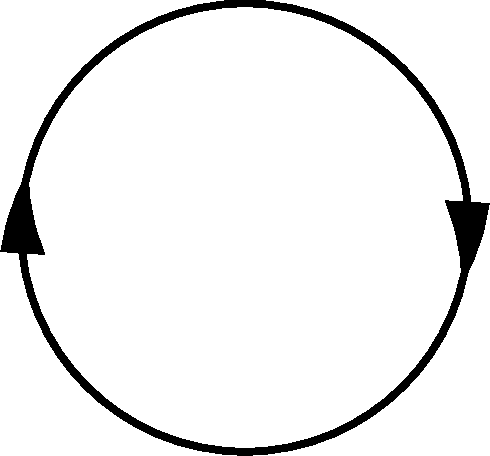
\includegraphics[width=0.7\linewidth]{loopT2.pdf}}
\end{minipage}
  column 1 \text{Tr} \ln \left(  column 1 \slashed{\partial}  column 1 \right) \nonumber\\
  column 1 \frac{y_t^4}{64 \pi^2} \left(\frac{2}{\bar{\epsilon}}  column 1 \ln \frac{y_t^2 F^2}{2 \mu^2}  column 1 \frac{3}{2}\right)  column 1 \,  column 1  \end{align}
  column 1  column 1  column 1  \begin{align}
\begin{minipage}[h]{0.1\linewidth}
\center{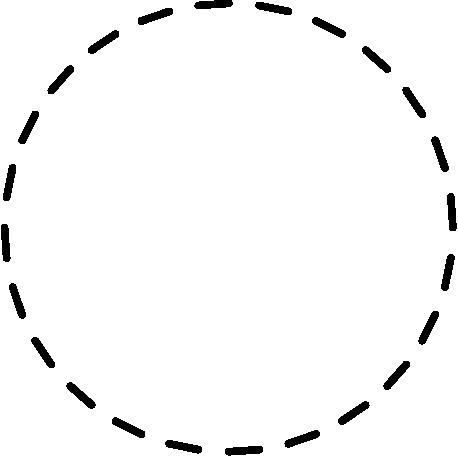
\includegraphics[width=0.7\linewidth]{loopH2.pdf}}
\end{minipage}
  column 1 \frac{1}{2} \text{Tr} \ln \left[\Box  column 1 \left(\frac{\lambda}{4}  column 1 \right)  column 1 \right] \nonumber\\
  column 1 \frac{9 \lambda^2}{64 \pi^2} \left(\frac{2}{\bar{\epsilon}}  column 1 \ln \frac{\lambda (F^4)''}{4 \mu^2}  column 1 \frac{3}{2}\right)\left(  column 1 {'2}  column 1 \frac{1}{3}  column 1 \right)  column 1 \,  column 1  \end{align}
  column 1  column 1   column 1  column 1  column 1  column 1   column 1     column 1  column 1  column 1  column 1  column 1  column 1  column 1  column 1  column 1 \cite{1412.3811}  column 1  
  column 1  column 1  column 1  column 1  column 1  column 1  column 1  column 1  column 1  column 1  column 1  column 1  column 1  column 1  column 1  column 1  column 1  column 1  column 1  column 1  column 1  column 1  column 1   column 1   column 1  column 1  column 1  column 1  column 1  column 1  column 1  column 1  column 1    column 1  column 1  column 1  column 1  column 1   column 1  column 1  column 1  column 1   column 1  column 1  column 1  column 1  column 1   column 1  column 1  
  column 1  column 1  column 1  column 1   column 1  column 1  column 1  column 1  column 1   column 1  column 1  column 1  column 1   column 1  column 1   column 1  column 1  column 1  column 1   column 1  column 1  column 1  column 1  column 1  column 1  column 1  column 1  column 1  column 1  column 1  column 1  column 1  column 1  
  column 1   column 1  column 1  column 1  column 1  column 1  column 1  column 1   column 1  column 1  column 1  column 1   column 1  column 1  column 1  column 1  column 1   column 1  column 1  column 1  column 1  column 1  column 1  column 1  column 1  column 1  column 1  column 1   column 1  column 1 \eg  column 1  column 1  column 1  column 1  column 1  column 1  column 1  column 1 \Eq \eqref{counterTerms}  column 1  column 1  column 1  column 1  column 1  column 1  column 1  column 1  column 1  column 1  column 1  column 1  column 1  column 1  column 1  column 1  column 1  column 1  column 1  column 1  column 1  column 1  column 1  column 1   column 1  column 1  column 1   
  column 1  column 1  column 1  column 1  column 1  column 1  column 1   column 1  column 1  column 1  column 1   column 1  column 1  column 1  column 1  column 1  column 1  column 1  column 1  column 1   column 1  column 1  column 1  column 1   column 1  column 1  column 1 \ref{table}  column 1   column 1  column 1  column 1   column 1  column 1  column 1  column 1  column 1  column 1  column 1  column 1  column 1   column 1  column 1  column 1 \Eqs  column 1 \ref{FieldTransform2}  column 1 \ref{NofH}  column 1  column 1   column 1   column 1  column 1  column 1  column 1   column 1  column 1  column 1  column 1  column 1  column 1  column 1  column 1  column 1  column 1  column 1  column 1  column 1  column 1  column 1  column 1   column 1   column 1  column 1  column 1  column 1  column 1  column 1  column 1  column 1  column 1  column 1  column 1  column 1  column 1  column 1  column 1   column 1  column 1  column 1  column 1  column 1  column 1  column 1  column 1  column 1  column 1  column 1  column 1  column 1  column 1  column 1  column 1  column 1     column 1  column 1  column 1  column 1  column 1  column 1 \Eq \eqref{mu}  column 1  column 1  column 1   column 1  column 1  column 1 \ref{table}  column 1  column 1   column 1  column 1  column 1  column 1  column 1  column 1  column 1  column 1   column 1  column 1  column 1  column 1  column 1  column 1  column 1  column 1   column 1  column 1  column 1   column 1  column 1  column 1  column 1  column 1  column 1  column 1  column 1  column 1  column 1  column 1  column 1  column 1  column 1  column 1  column 1  column 1 \ref{table2}  column 1   	\begin{table}
	\begin{center}
		
		\caption{  caption  caption  caption  caption  caption  caption  caption  caption  caption  caption }
		\label{table2}
		\end{center}
	\end{table}



  column 1  column 1  column 1  column 1  column 1  column 1  column 1  column 1  column 1  column 1   column 1  column 1  column 1  column 1  column 1  column 1  column 1  column 1     column 1  column 1   column 1  column 1  column 1  column 1  column 1  column 1  column 1  column 1    column 1 \ie  column 1  column 1  column 1  column 1  column 1  column 1  column 1  column 1  column 1  column 1  column 1  column 1  column 1  column 1  column 1  column 1  column 1  column 1  column 1  column 1  column 1  column 1  column 1   column 1  column 1  column 1  column 1  column 1  column 1  column 1  column 1  column 1 \ie  column 1  column 1  column 1  column 1   column 1  column 1  column 1  column 1  column 1  column 1  column 1    column 1  column 1  column 1 \footnote
%
{We assume that new heavy particles, if they exist at all, have no impact on inflation beyond changing the $\beta$-functions. We also ignore all quadratic divergences associated with these particles (see \cite{Bardeen:1995kv, 0708.3550, 1303.7244}).}
%

  column 1   column 1  column 1  column 1  column 1  column 1  column 1  column 1  column 1  column 1  column 1  column 1  column 1  column 1   column 1   column 1  column 1  column 1   column 1  column 1  column 1  column 1  
  column 1  column 1  column 1  column 1   column 1   column 1  column 1  column 1  column 1  column 1  column 1  column 1  column 1  column 1    column 1  column 1  column 1  column 1  column 1 \footnote
%
{One can obtain this result by expressing the one-loop contribution to the vertex function in terms of the physical coupling, which is defined in the momentum dependent subtraction scheme at the scale $\mu$ and thus accounts for decoupling of heavy degrees of freedom for $\mu \ll m$.} 
%

  column 1  column 1  column 1  column 1  column 1  column 1   column 1  column 1  column 1   column 1   column 1  
  column 1  column 1  column 1  column 1   column 1  column 1 \Eqs \eqref{deltaLambdaMetric}  column 1 \eqref{deltaLambdaPalatini}  column 1  column 1  column 1  column 1  column 1  column 1  column 1  column 1  column 1  column 1  column 1  column 1  column 1  column 1   column 1     column 1  column 1  column 1  column 1   column 1  column 1  column 1  column 1  column 1  column 1  column 1  column 1  column 1  column 1  column 1  column 1   column 1  column 1  column 1  column 1  column 1  column 1  column 1  column 1  column 1  column 1   column 1  column 1  column 1  column 1  column 1  column 1  column 1  column 1  column 1  column 1 \eqref{deltaLambdaPalatini}  column 1  column 1  column 1  column 1  column 1  column 1  column 1  column 1  column 1  column 1  column 1  column 1  column 1  column 1  column 1  column 1  column 1   column 1  column 1  column 1  column 1  column 1  column 1  column 1  column 1  column 1  column 1  column 1  column 1  column 1  column 1  column 1  column 1   column 1  column 1  column 1  column 1  column 1  column 1  column 1  column 1  column 1  column 1   column 1  column 1  column 1  column 1  column 1  column 1  column 1  column 1  column 1  column 1  column 1  column 1  column 1  column 1 \eqref{deltaBetaPalatini} \cite{1308.2627, 1402.1476}  column 1 \footnote
%
{In our approach, we exclude higher-dimensional operators that do not respect the approximate shift symmetry $\chi \rightarrow \chi + $const of the potential $U(\chi)$. Adding those can easily make inflation impossible (or change inflationary predictions) \cite{1712.08471, 1904.05699}. In contrast, quantum corrections that are generated by the theory itself are small \cite{1712.04874}.}
%
  column 1  column 1  column 1  column 1 \eqref{deltaLambdaPalatini}  column 1  column 1  column 1  column 1   
\section{  section  section  section  section  section  section }
\label{sec:connection}
  column 1  column 1  column 1  column 1  column 1  column 1  column 1  column 1  column 1  column 1  column 1  column 1  column 1  column 1  column 1  column 1  column 1  column 1    column 1  column 1  column 1  column 1  column 1  column 1  column 1  column 1  column 1  column 1  column 1  column 1  column 1  column 1  column 1  column 1  column 1  column 1  column 1  column 1  column 1  column 1  column 1    column 1  column 1  column 1  column 1  column 1  column 1  column 1  column 1   column 1  column 1  column 1  column 1  column 1  column 1  column 1   column 1  column 1  column 1  column 1  column 1   column 1  column 1  column 1  column 1  column 1  column 1  column 1  column 1  column 1  column 1    column 1   column 1  column 1  column 1  column 1  column 1  column 1  column 1  column 1  column 1  column 1  column 1  column 1  column 1  column 1  column 1  column 1  column 1     column 1  column 1  column 1  column 1   column 1  column 1 \Eq \eqref{slowRollParameters}  column 1  column 1  column 1  column 1  column 1 \eqref{normalization}  column 1  column 1 \Eq \eqref{NofH}  column 1  column 1  
  column 1  column 1   column 1  column 1   column 1  column 1  column 1   column 1  column 1  column 1  column 1   column 1  column 1  column 1  column 1  column 1  column 1  column 1  column 1  column 1  column 1  column 1  column 1    column 1  column 1  column 1  column 1  column 1   column 1 \footnote
%
{We thank Fedor Bezrukov for kindly providing us with a script to do so. The script computes the running of the Standard Model couplings  in the $\overline{\text{MS}}$-scheme. It uses two-loop matching of physical and $\overline{\text{MS}}$ parameters  \cite{1507.08833} and three-loop RG evolution of coupling constants \cite{1205.2892} (see also \cite{1205.2893,1205.6497,1307.3536}). As an input, we use $\alpha_s(M_Z)=0.1181$ and $m_h=125.1\,$GeV. The influence of $\xi$ on the running is negligible \cite{0904.1537}, and we do not consider it.}
%
  column 1  column 1  column 1  column 1  column 1  column 1  column 1  
  column 1  column 1  column 1  column 1  column 1  column 1  column 1   column 1   column 1   column 1  column 1  column 1  column 1  column 1  column 1  column 1  column 1  column 1  column 1  column 1  column 1  column 1  column 1  column 1  column 1  column 1  column 1  column 1  column 1  column 1  column 1  column 1   column 1  column 1  column 1  column 1  column 1  column 1  column 1  column 1  column 1  column 1  column 1  column 1 \cite{Tanabashi:2018oca}  column 1  column 1  column 1   column 1  column 1  column 1  column 1  column 1   column 1  column 1 \Eqs  column 1 \ref{mu}  column 1 \eqref{runningCoupling}  column 1  column 1 \eqref{xiOfLambda}  column 1  column 1  
  column 1   column 1  column 1  column 1  column 1  column 1  column 1  column 1  column 1  column 1  column 1   column 1   column 1   column 1   column 1  column 1  column 1  column 1  column 1   column 1  column 1  column 1  column 1  column 1  column 1 \eqref{Yt}  column 1  column 1  column 1  column 1  column 1  column 1   column 1   column 1  column 1  column 1  column 1  column 1  column 1  column 1   column 1 \ie  column 1  column 1  column 1  column 1 \Eq \eqref{NofH}  column 1  column 1  column 1  column 1  column 1  column 1  column 1  column 1  column 1  column 1  column 1  column 1  column 1  column 1  column 1   \Eq \eqref{xiEquation}  column 1  column 1   column 1  column 1   column 1  column 1  column 1  column 1  column 1  column 1  column 1  column 1  column 1  column 1  column 1  column 1  column 1  column 1  column 1  column 1  column 1  column 1  column 1  column 1  column 1  column 1  column 1  column 1 \footnote
%
{In fact, one should impose the slightly stricter criterion of avoiding eternal inflation because otherwise the classical treatment is not valid. Since it will turn out in the numerical analysis that $\diff U/\diff \chi$  never comes close to $0$, this distinction is inessential.}
% 

  column 1  column 1  column 1  column 1  column 1  column 1  column 1  column 1  column 1  column 1  column 1  column 1  column 1  column 1  column 1  column 1  column 1   column 1  column 1   column 1  
  column 1  column 1 \Eqs \eqref{Potential}  column 1 \eqref{mu}  column 1  column 1   column 1  column 1  column 1  column 1  column 1  column 1  column 1  column 1   column 1  column 1  column 1  column 1  column 1  
  column 1  column 1 \Eq \eqref{xiOfLambda}  column 1  column 1 \footnote
%
{This bound only refers to inflation on the plateau. Other scenarios, such as hilltop inflation, can allow for smaller values of $\xi$; see \cite{1709.07853, 1802.09299}.}
%

  column 1  column 1  column 1   column 1   column 1  %It does not arise from collider physics but from the requirement that inflation is possible. 
  column 1  column 1  column 1  column 1  column 1  column 1 \Eq \eqref{NofH}  column 1  column 1  column 1  column 1  column 1  column 1   column 1  column 1  column 1  column 1   column 1  column 1  column 1  column 1  column 1  column 1  column 1  column 1  column 1  column 1  column 1  column 1  column 1 \Eq \eqref{xiMinAnalytic}  column 1  column 1  column 1  column 1  column 1 \ref{app}  column 1  column 1  
  column 1  column 1   column 1   column 1 \footnote
%
{A lower bound on $\xi$ has already been discussed in a different setup in \cite{1709.07853}. There, no connection was made to low-energy data of the Standard Model, i.e., $\lambda_0$, $b$ and $q$ were treated as free parameters. Moreover, only positive values of $\lambda_0$ were considered. This led to $\xi_{\text{min}}\approx 6\cdot 10^6$ \cite{1709.07853}.}
%


  column 1  column 1  column 1  column 1  column 1   column 1  column 1  column 1  column 1  column 1  column 1  column 1   column 1  column 1  column 1  column 1  column 1  column 1  column 1  column 1  column 1  column 1  column 1  column 1  column 1  column 1  column 1  column 1  column 1 \cite{1509.04044}   column 1  column 1  column 1 \cite{1810.01772}    column 1  column 1  column 1  column 1  column 1 \cite{Tanabashi:2018oca}  column 1  column 1  column 1  column 1  column 1  column 1  column 1  column 1  column 1  column 1  column 1  column 1  column 1  column 1 \cite{1411.1923}  column 1  column 1  column 1  column 1  column 1  column 1  column 1  column 1  column 1  column 1   column 1  column 1 \eg \cite{1412.3649, 1801.03944}  column 1  column 1  column 1  column 1  column 1   column 1  column 1  column 1  column 1  column 1  column 1  column 1  column 1  column 1  column 1  column 1   column 1  column 1  column 1  column 1  column 1   column 1   column 1  column 1  column 1  column 1  column 1  column 1  column 1  column 1  column 1   column 1  column 1    column 1  column 1  
  column 1  column 1  column 1  column 1  column 1  column 1  column 1  column 1  column 1  column 1  column 1  column 1  column 1  column 1  column 1  column 1  column 1  column 1  column 1  column 1  column 1  column 1  column 1  column 1   column 1     column 1  column 1  column 1  column 1  column 1  column 1  column 1 \Eq \eqref{xiEquation}  column 1  column 1  column 1 \fig \ref{sfig:xiOfLambda0}  column 1  column 1  column 1  column 1   column 1  column 1  column 1  column 1   column 1  column 1  column 1  column 1   column 1  column 1  column 1  column 1  column 1  column 1   column 1  column 1   column 1  column 1  column 1  column 1   column 1  column 1  column 1  column 1  column 1  column 1  column 1  column 1  column 1  column 1  
  column 1  column 1  column 1   column 1   column 1  column 1  column 1  column 1   column 1  column 1  column 1   column 1  column 1  column 1  column 1  column 1   column 1  column 1  column 1  column 1  column 1  column 1  column 1 \eqref{topMassMax}  column 1  column 1  column 1   column 1     column 1  column 1  column 1  column 1  column 1  column 1  column 1  column 1  column 1  column 1  column 1  column 1  column 1  column 1  column 1   column 1  column 1  column 1  column 1   column 1  column 1  column 1 \eqref{deltaLambdaPalatini}  column 1  column 1  column 1  column 1 \eqref{upperXi}  column 1  column 1  column 1  column 1  column 1  column 1 \eqref{xiMinAnalytic}  column 1   column 1  column 1  column 1  column 1 \eqref{topMassMax}  column 1  column 1  column 1  column 1  column 1  column 1  column 1  column 1  column 1   column 1  column 1  column 1  column 1  column 1  column 1  column 1  column 1  column 1  column 1  column 1  column 1  column 1  column 1  column 1 \footnote
%
{It is an interesting numerical coincidence that $\delta \lambda$, the magnitude of which is essentially given by a loop factor, and values of $\lambda$ that can support inflation are of the same order of magnitude.}
%
  column 1  column 1  column 1  column 1  column 1   column 1  column 1  column 1  column 1  column 1  column 1  column 1  column 1  column 1   column 1  column 1   column 1  column 1 \Eq \eqref{deltaLambdaPalatini}  column 1  column 1  column 1 \eqref{topMassMax}  column 1  column 1   column 1  column 1  column 1  column 1  column 1  column 1  
  column 1  column 1  column 1  column 1  column 1  column 1  column 1   column 1     column 1  column 1  column 1  column 1  column 1  column 1  column 1  column 1  column 1  column 1  column 1  column 1  column 1  column 1   column 1  column 1  column 1   column 1  column 1  column 1   column 1  column 1  column 1  column 1  column 1  column 1  column 1   column 1   column 1  column 1  column 1   column 1   column 1  column 1  column 1 \eqref{xiMin}  column 1 \eqref{topMassMax}  column 1  column 1   column 1   column 1  column 1  column 1  column 1  column 1  column 1  column 1   column 1  column 1  column 1  column 1   column 1  column 1  column 1   column 1  column 1  column 1  column 1  column 1 \Eq \eqref{deltaLambdaPalatini}  column 1 \ie   column 1  column 1  column 1  column 1  column 1  column 1   \begin{figure}
	\centering 
	\begin{subfigure}{0.6\textwidth}
		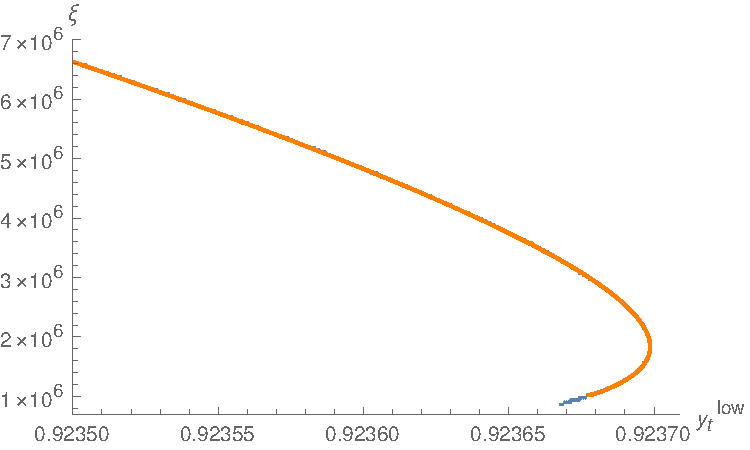
\includegraphics[width=\textwidth]{xiOfYt0.pdf}
	\end{subfigure}
	\hspace{0.02\textwidth}
	\caption{  caption  caption  caption   caption  caption  caption  caption  caption  caption  caption  caption   caption  caption  caption  caption  caption  caption  caption  caption  caption  caption  caption  caption  caption   caption  caption  caption  caption  caption  caption  caption  caption  caption  caption  caption  caption  caption  caption  caption  caption  caption  caption  caption  caption  caption  caption  caption   caption  caption  caption  caption }
			\label{sfig:xiOfLambda0}
\end{figure} 

  column 1  column 1  column 1  column 1  column 1  column 1  column 1  column 1  column 1  column 1  column 1  column 1  column 1  column 1  column 1  column 1   column 1  column 1  column 1  column 1  column 1   column 1  column 1  column 1  column 1  column 1  column 1  column 1  column 1  column 1 \cite{0812.4950, 0904.1537}  column 1  column 1  column 1  column 1  column 1  column 1  column 1  column 1  column 1    column 1  column 1  column 1  column 1  column 1  column 1 \eqref{mu}  column 1  column 1  column 1  column 1  column 1  column 1  column 1  column 1  column 1  column 1  column 1  column 1  column 1 \ie  column 1  column 1  column 1  column 1  column 1  column 1  column 1  column 1  column 1  column 1  column 1  column 1  column 1  column 1  column 1  column 1   
  column 1  column 1  column 1  column 1  column 1  column 1  column 1  column 1  column 1 \ref{table}  column 1  column 1  column 1   column 1  column 1  column 1   column 1  column 1 \Eq \eqref{NofH}  column 1  column 1  column 1  column 1  column 1  column 1 \eqref{normalization}  column 1  column 1  column 1 \Eq \eqref{xiOfLambda}

  column 1  column 1  column 1  column 1  column 1   column 1  column 1   column 1  column 1   column 1  column 1  column 1  column 1  column 1  column 1  column 1  \eqref{runningCoupling}  column 1  column 1  column 1   column 1  column 1 \Eq \eqref{mu}  column 1  column 1  column 1  column 1   column 1  column 1  column 1  column 1  column 1   column 1     column 1  column 1  column 1  column 1  column 1   column 1  column 1  column 1  column 1 \eqref{runningCondition}  column 1  column 1  column 1 \eqref{lambdaLowerBound}  column 1  column 1  column 1  column 1  column 1  column 1  column 1    column 1  column 1  column 1  column 1  column 1   column 1  column 1   column 1   column 1   column 1  column 1  column 1   column 1  column 1  column 1  column 1   column 1  column 1  column 1  column 1  column 1  column 1  column 1  
  column 1  column 1  column 1   column 1   column 1  column 1  column 1  column 1  column 1  column 1  column 1  column 1  column 1  column 1  column 1  column 1    column 1  column 1  column 1 \Eq \eqref{topMassMax}  column 1  column 1   column 1  column 1  column 1  column 1  column 1 \eqref{topMassMaxMetric}  column 1  column 1  column 1   column 1   column 1   column 1  column 1  column 1  column 1  column 1  column 1  column 1  column 1  column 1  column 1  column 1  column 1  column 1  column 1  column 1  column 1  column 1  column 1  column 1  column 1  column 1 \Eq \eqref{topMassMaxMetric}  column 1  column 1  column 1  column 1  column 1  column 1     column 1  column 1  column 1  column 1  column 1  column 1  column 1  column 1  column 1  column 1  column 1  column 1   column 1  column 1  column 1 \eqref{topMassMaxMetric}  column 1  column 1   column 1  column 1  column 1   column 1  column 1 \Eq \eqref{deltaLambdaMetric}  column 1  column 1   column 1  column 1  column 1  column 1  column 1 \cite{1008.5157, 1403.6078, 1412.3811}  column 1  column 1  column 1  column 1  column 1  column 1  column 1  column 1  column 1  column 1  column 1  column 1  column 1  column 1  column 1  column 1 \eqref{topMassMaxMetric}  column 1  column 1  column 1  column 1  column 1  column 1  column 1  column 1  column 1  column 1  column 1  column 1  column 1   column 1  column 1  column 1  column 1  column 1  column 1  column 1  column 1  column 1  column 1  column 1  column 1  column 1  column 1  column 1  column 1  column 1   
\section{  section  section }
\label{sec:conclusion}
  column 1  column 1  column 1  column 1  column 1  column 1  column 1 \cite{0710.3755}  column 1  column 1  column 1 \cite{0803.2664}  column 1  column 1  column 1  column 1  column 1  column 1  column 1  column 1  column 1  column 1  column 1  column 1  column 1  column 1  column 1  column 1  column 1  column 1  column 1  column 1  column 1  column 1  column 1  column 1  column 1  column 1   column 1  column 1  column 1  column 1  column 1  column 1  column 1  column 1  column 1  column 1  column 1  column 1 \cite{1012.2900}  column 1  column 1  column 1  column 1  column 1  column 1  column 1  column 1  column 1  column 1  column 1  column 1  column 1  column 1  column 1  column 1  column 1  column 1   column 1  column 1  column 1  column 1  column 1  column 1 \cite{1008.5157}  column 1  column 1  column 1  column 1  column 1  column 1  column 1  column 1  column 1  column 1  column 1  column 1  column 1     column 1  column 1  column 1  column 1  column 1  column 1  column 1  column 1   column 1  column 1  column 1  column 1  column 1  column 1  column 1  column 1  column 1  column 1  column 1  column 1  column 1  column 1  column 1   column 1  column 1  column 1  column 1  column 1  column 1  column 1  column 1  column 1  column 1  column 1  column 1  column 1  column 1  column 1  column 1  column 1  column 1  column 1  column 1  column 1  column 1   column 1  column 1  column 1  column 1  column 1  column 1  column 1  column 1  column 1   column 1  column 1   column 1  column 1   column 1  column 1  column 1  column 1  column 1  column 1   column 1  column 1  column 1  column 1  column 1  column 1  column 1  column 1  column 1  column 1  column 1 \cite{1904.05237, 1905.02302}  column 1 \footnote
	%
{CMS and ATLAS  have measured $m_{t}^{\text{pole}}=170.5\pm0.8\,\text{GeV}$ \cite{1904.05237} and $m_{t}^{\text{pole}}=171.1\pm1.2\,\text{GeV}$ \cite{1905.02302}, respectively.}
	%
  column 1  column 1  column 1  column 1  column 1  column 1  column 1  column 1  column 1  column 1   column 1   column 1  column 1  column 1  column 1  column 1   column 1  column 1  column 1  column 1     column 1  column 1  column 1  column 1  column 1  column 1  column 1  column 1  column 1   column 1  column 1  column 1  column 1  column 1  column 1  column 1  column 1  column 1  column 1  column 1  column 1  column 1  column 1  column 1  column 1  column 1  column 1  column 1  column 1  column 1  column 1  column 1  column 1  column 1  column 1  column 1   column 1  column 1  column 1  column 1   column 1  column 1 \ref{xiMin}  column 1  column 1  column 1 \ref{upperXi}  column 1  column 1  column 1     column 1  column 1  column 1  column 1  column 1  column 1  column 1  column 1  column 1  column 1  column 1  column 1  column 1  column 1  column 1  column 1  column 1  column 1   column 1  column 1  column 1  column 1  column 1  column 1  column 1  column 1  column 1  column 1  column 1  column 1  column 1  column 1   column 1  column 1  column 1  column 1  column 1  column 1  column 1  column 1  column 1  column 1  column 1  column 1   column 1  column 1  column 1  column 1  column 1  column 1  column 1  column 1  column 1  column 1  column 1   column 1  column 1  column 1  column 1  column 1  column 1  column 1  column 1  column 1  column 1  column 1  column 1  column 1  column 1  column 1  column 1 \cite{Froggatt:1995rt}  column 1  column 1  column 1  column 1  column 1 \cite{0912.0208}  column 1     column 1  column 1  column 1  column 1  column 1  column 1  column 1  column 1  column 1  column 1  column 1  column 1   column 1 \cite{2001.09088}  column 1  column 1  column 1  column 1  column 1  column 1  column 1  column 1  column 1  column 1  column 1  column 1  column 1  column 1  column 1  column 1  column 1  column 1  column 1  column 1  column 1  column 1 \eqref{action_full}  column 1   column 1  column 1  column 1  column 1  column 1  column 1  column 1  column 1  column 1  column 1  column 1  column 1  column 1  column 1  column 1  column 1  column 1  column 1  column 1  column 1  column 1  column 1  column 1  column 1  column 1  column 1  column 1  column 1  column 1  column 1  column 1  column 1  column 1  column 1  column 1  column 1  column 1  column 1  column 1  column 1  column 1  column 1  column 1  column 1  column 1  column 1 \cite{2001.09088}  column 1     column 1  column 1  column 1  column 1  column 1  column 1  column 1  column 1  column 1  column 1  column 1  column 1  column 1  column 1  column 1  column 1  column 1  column 1  column 1  column 1  column 1  column 1  column 1  column 1  column 1  column 1  column 1  column 1  column 1  column 1  column 1  column 1  column 1  column 1  column 1 \cite{Asaka:2005an, Asaka:2005pn}  column 1  column 1  column 1  column 1  column 1  column 1  column 1  column 1  column 1  column 1  column 1  column 1  column 1  column 1  column 1  column 1  column 1  column 1  column 1  column 1  column 1  column 1  column 1  column 1 \cite{1005.3497, 1010.1415, 1103.5963}  column 1  column 1  column 1  column 1  column 1  column 1  column 1  column 1  column 1  column 1  column 1  column 1  column 1   \section*{  section  section }
  column 1  column 1  column 1  column 1  column 1  column 1  column 1  column 1  column 1  column 1  column 1  column 1  column 1  column 1  column 1  column 1  column 1  column 1  column 1  column 1  column 1  column 1  column 1  column 1  column 1  \underline{ }  column 1   \appendix

\section{  section  section  section  section }
\label{app}
  column 1  column 1  column 1  column 1  \ref{sec:connection}  column 1  column 1  column 1  column 1  column 1  column 1   column 1  column 1  column 1  column 1   column 1  column 1  column 1  column 1  column 1  column 1 \Eq \eqref{NofH}  column 1  column 1  column 1  column 1   column 1  column 1  column 1  column 1   column 1  column 1  column 1  column 1  column 1   column 1   column 1  column 1  column 1  column 1  column 1  column 1  column 1  column 1  column 1  column 1  column 1  column 1  column 1  column 1  column 1    column 1  column 1  column 1   column 1  column 1  column 1  column 1 \Eq \eqref{normalization}  column 1   column 1  column 1  column 1  column 1  column 1  column 1  column 1  column 1  column 1   column 1  column 1  column 1   column 1   column 1  column 1  column 1  column 1  column 1  column 1  column 1  column 1   column 1  column 1 \ref{table}  column 1  column 1  column 1  column 1  column 1  column 1   column 1  column 1  column 1  column 1  column 1  column 1  column 1   
  column 1  column 1  column 1  column 1  column 1   column 1  column 1  column 1   column 1 \footnote
%
{We use Mathematica \cite{mathematica} for the numerical analysis.}
%
  column 1  column 1  column 1  column 1  column 1  column 1  column 1  column 1  column 1  column 1  column 1  column 1  column 1  column 1  column 1 \eqref{xiEquation}  column 1  column 1  column 1   column 1  column 1  column 1  column 1  column 1  column 1  column 1  column 1  column 1  column 1  column 1  column 1   column 1  column 1 \Eq \eqref{xiMin}  column 1  column 1  column 1  column 1  column 1  column 1  column 1  column 1  column 1  column 1  column 1  column 1  column 1  column 1  column 1  column 1  column 1  column 1  column 1  column 1  column 1  \fig \ref{sfig:xiOfLambda0}  column 1  column 1  column 1  column 1  column 1  column 1  column 1  column 1  column 1  column 1  column 1  column 1  column 1  column 1   column 1  column 1  column 1  column 1  column 1  column 1  column 1  column 1 \eqref{topMassMax}  column 1  column 1  column 1  column 1     column 1  column 1  column 1  column 1  column 1  column 1 \fig \ref{sfig:epsilonOfLambda0}  column 1  column 1  column 1  column 1   column 1  column 1  column 1  column 1   column 1  column 1  column 1  column 1  column 1  column 1 \Eq \eqref{xiOfLambda}  column 1  column 1  column 1  column 1   column 1  column 1    column 1  column 1  column 1   column 1  column 1  column 1   column 1  column 1  column 1 \ref{table}  column 1  column 1  column 1  column 1  column 1  column 1   \begin{figure}
	\centering 
	\begin{subfigure}{0.6\textwidth}
		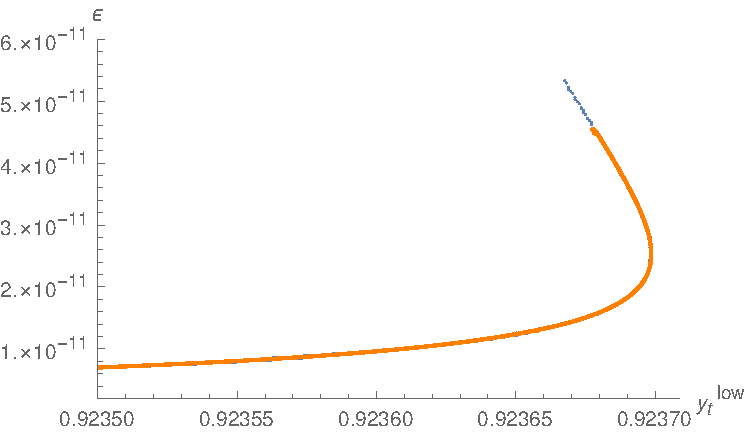
\includegraphics[width=\textwidth]{epsilonOfYt0.pdf}
	\end{subfigure}
		\caption{  caption  caption  caption   caption  caption  caption  caption  caption  caption  caption  caption   caption  caption  caption  caption  caption  caption  caption  caption  caption  caption  caption  caption  caption  caption  caption  caption  caption \fig \ref{sfig:xiOfLambda0}  caption }
				\label{sfig:epsilonOfLambda0}
\end{figure}

\bibliographystyle{JHEP}
\bibliography{inflationBib}

\end{document}
